\subsubsection{Радуга}
\label{sec:rainbow}

\newcommand{\drawRainbow}[2][1]{
    \tkzInit[xmin=-0.4, ymin=-1.5*#1, xmax=2.1, ymax=1.1*#1]
    \tkzClip
    
    \tkzDefPoint(0,0){R}
    \tkzDefPoint(1,0){C}
    
    \foreach \x in {-0.02,-0.04,...,-1} {
%        \tkzSetUpLine[gray]

        \tkzDefPoint(-0.5,\x){A}
        \tkzDefPoint(0,\x){B}
        
        \tkzInterLC(B,A)(C,R) 
        \tkzGetPoints{R1}{x}
        
        \tkzDrawSegment[gray](A,R1)
        
        \tkzFindAngle(A,R1,C) 
        \tkzGetAngle{ABC}
        
        \pgfmathparse{\ABC - 180}
        \pgfmathsetmacro\ALPHA{\pgfmathresult}
        
        \pgfmathparse{asin(sin(\ALPHA)/1.333)}
        \pgfmathsetmacro\BETA{\pgfmathresult}
        
        \tkzDefPointBy[homothety=center R1 ratio 1](R1) 
        \tkzGetPoint{R2}
        \foreach \i in {0,1,...,#2} {
            \tkzDefPointBy[rotation=center R1 angle -\BETA](C) 
            \tkzGetPoint{R1'}
            
            \tkzInterLC(R1,R1')(C,R) 
            \tkzGetPoints{x}{R2}
            
            \tkzDrawSegment[gray](R1,R2)
            
            \tkzDefPointBy[homothety=center R1 ratio 1](R2) 
            \tkzGetPoint{R1}
        }
        
        \tkzDefPointBy[rotation=center R1 angle -180 + \ALPHA](C) 
        \tkzGetPoint{L'}
        
        \tkzDefPointBy[homothety=center R1 ratio 1.5](L') 
        \tkzGetPoint{L}
        
        \tkzDrawSegment[gray](R2,L)
    }
        
    \tkzDefPoint(-0.5,0){A0}
    \tkzDefPoint(2,0){B0}
    \tkzDrawSegment[dotted, thick](A0,B0))
        
    \tkzDrawCircle[thick, black](C,R)
}
\def\drawRainbowDispersion(#1){% (count)
    \tkzInit[xmin=-0.4, ymin=-1.5, xmax=2.1, ymax=1.1]
    \tkzClip
    
    \tkzDefPoint(0,0){R}
    \tkzDefPoint(1,0){C}
    
    \foreach \n in {1.332,1.334,...,1.345} {
        \tkzSetUpLine[gray]

        \pgfmathparse{sqrt((1 + #1)^2 -\n^2)/sqrt(2 * #1 + #1 * #1)}
        \pgfmathsetmacro\x{\pgfmathresult}

    
        \tkzDefPoint(-0.5,-\x){A}
        \tkzDefPoint(0,-\x){B}
        
        \tkzInterLC(B,A)(C,R) 
        \tkzGetPoints{R1}{x}
        
        \tkzDrawSegment(A,R1)
        
        \tkzFindAngle(A,R1,C) 
        \tkzGetAngle{abc}
        
        \pgfmathparse{\abc - 180}
        \pgfmathsetmacro\ALPHA{\pgfmathresult}
            
        \pgfmathparse{asin(sin(\ALPHA)/\n)}
        \pgfmathsetmacro\BETA{\pgfmathresult}
        
        \tkzDefPointBy[homothety=center R1 ratio 1](R1)
        \tkzGetPoint{R2}
        
        \foreach \i in {0,1,...,#1} {
            \tkzDefPointBy[rotation=center R1 angle -\BETA](C) 
            \tkzGetPoint{R1'}
            
            \tkzInterLC(R1,R1')(C,R) 
            \tkzGetPoints{x}{R2}
            
            \tkzDrawSegment(R1,R2)
            
            \tkzDefPointBy[homothety=center R1 ratio 1](R2) 
            \tkzGetPoint{R1}
        }
                
        \pgfmathparse{-180+\ALPHA}
        \pgfmathsetmacro\r{\pgfmathresult}
        
        \tkzDefPointBy[rotation=center R1 angle \r](C) 
        \tkzGetPoint{L'}
        
        \tkzDefPointBy[homothety=center R1 ratio 1](L') 
        \tkzGetPoint{L}
        
        \tkzDrawSegment(R1,L)
    }
        
    \tkzDefPoint(-0.5,0){A0}
    \tkzDefPoint(2,0){B0}
    \tkzDrawSegment[dotted, thick](A0,B0))
        
    \tkzDrawCircle[thick, black](C,R)
}

Радуга~--- событие проявления преломления (рефракции) и отражения солнечного света, в каплях воды, распыленных в воздуха. Наблюдается в виде ярких разноцветных колец, перпендикулярных прямой \textsl{Солце -- наблюдатель}, с центром на ней. 

Стоит обратить внимание на возможность обобщения данной формулировки. Излучение может быть монохромным, тогда радуга будет также монохромна. Для появления радуги необязательно наличие воздуха. Данного эффекта можно достичь, распыляя воду в космосе~--- без атмосферы и гравитации. Также радуга может наблюдаться во взвеси стеклянных шариков или капель любой другой прозрачной для рассматриваемого излучения жидкости.

Рассмотрим детальнее, как формируются радужные кольца. Для упрощения расчетов солнечный свет можно считать параллельным фронтом с выделенным направлением, а капли воды с достаточной точностью сферическими. 

\begin{wrapfigure}[13]{r}{0.47\tw}
    \vspace{-1.5pc}
    \tikzsetnextfilename{rainbow-scheme}
\begin{tikzpicture}[
    scale=2,
    arrow/.style 2 args={
        postaction=decorate,
        decoration={
            markings, 
            mark=at position #2 with {\arrow{#1}}
        } 
    }
]
    \tkzInit[xmin=-0.55, ymin=-1.2, xmax=2.15, ymax=1.15]
    \tkzClip
    
    \tkzDefPoint(0,0){R}
    \tkzDefPoint(1,0){C}

    \tkzDefPoint(-0.5,0.8){A}
    \tkzDefPoint(0,0.8){B}
    
    \tkzInterLC(B,A)(C,R) 
    \tkzGetPoints{x}{R1}
    
    \tkzFindAngle(A,R1,C) 
    \tkzGetAngle{ABC}
    
    \pgfmathparse{180 - \ABC}
    \pgfmathsetmacro\ALPHA{\pgfmathresult}
    
    \pgfmathparse{asin(sin(\ALPHA)/1.333)}
    \pgfmathsetmacro\BETA{\pgfmathresult}
    
    \tkzDefPointBy[rotation=center R1 angle \BETA](C) 
    \tkzGetPoint{R1'}
    \tkzInterLC(R1,R1')(C,R) 
    \tkzGetPoints{R2}{x}
    
    \tkzDefPointBy[rotation=center R2 angle \BETA](C) 
    \tkzGetPoint{R2'}
    \tkzInterLC(R2,R2')(C,R) 
    \tkzGetPoints{R3}{x}
    
    \tkzDefPointBy[rotation=center R3 angle \BETA](C) 
    \tkzGetPoint{R3'}
    \tkzInterLC(R3,R3')(C,R) 
    \tkzGetPoints{R4}{x}
    
    \tkzDefPointBy[rotation=center R4 angle 180-\ALPHA](C) 
    \tkzGetPoint{L}
    
    \tkzDefPoint(-0.5,0){A0}
    \tkzDefPoint(2,0){B0}
    \tkzDrawSegment[dash dot, thick](A0,B0)
%    
    \tkzDrawSegments[arrow={latex}{0.5}](R1,R2 R2,R3 R3,R4 R4,L)
    \tkzDrawSegments[arrow={latex}{0.7}](A,R1)
    \tkzDrawLines[dashed](C,R2 C,R3)
    
    \tkzMarkAngle[line width = 0.15pt, size=0.01](C,R1,R2) % костыль для расстояния между дугами
    \tkzMarkAngles[size = 0.25](C,R1,R2 C,R2,R3 C,R3,R4)
    \tkzMarkAngles[size = 0.3](R1,R2,C R2,R3,C R3,R4,C)
    \tkzLabelAngles[pos=0.4, fill=white, inner sep=1pt](C,R1,R2 C,R2,R3 C,R3,R4 R1,R2,C R2,R3,C R3,R4,C){\footnotesize $\beta$}
    
    
    \tkzDefPointBy[homothety=center R1 ratio -0.5](C) \tkzGetPoint{C1}
    \tkzDefPointBy[homothety=center R2 ratio -0.5](C) \tkzGetPoint{C2}
    \tkzDefPointBy[homothety=center R3 ratio -0.5](C) \tkzGetPoint{C3}
    \tkzDefPointBy[homothety=center R4 ratio -.15](C) \tkzGetPoint{C4}
    
    \tkzDrawLines[dashed](C,C1 C,C4)
    \tkzMarkAngles[size=0.15, arc=ll](C1,R1,A L,R4,C4)
    \tkzLabelAngles[pos=0.3,font=\footnotesize](C1,R1,A L,R4,C4){$\alpha$}
    
    \tkzDefPointBy[rotation=center R1 angle -90](C) \tkzGetPoint{T1}
    \tkzDefPointBy[rotation=center R2 angle  90](C) \tkzGetPoint{T2}
    \tkzDefPointBy[rotation=center R3 angle  90](C) \tkzGetPoint{T3}
    \tkzDefPointBy[rotation=center R4 angle  90](C) \tkzGetPoint{T4}
    
    
    \tkzMarkRightAngles[size=0.1](T1,R1,C T2,R2,C2 T3,R3,C3 C,R4,T4)
    
    \tkzInterLL(R4,L)(A,R1)
    \tkzGetPoint{W}
    \tkzMarkAngle[line width = 0.2pt, size=0.01](C,R1,R2) % костыль для расстояния между дугами
    \tkzMarkAngle[arc=lll, size=0.15](R1,W,L)
    \tkzLabelAngle[pos=0.3, font=\footnotesize](R1,W,L){$\omega$}
    
    \tkzDefMidPoint(A,R1)  \tkzGetPoint{M0}
    \tkzDefMidPoint(R1,R2) \tkzGetPoint{M1}
    \tkzDefMidPoint(R2,R3) \tkzGetPoint{M2}
    \tkzDefMidPoint(R3,R4) \tkzGetPoint{M3}
    \tkzDefMidPoint(R4,L)  \tkzGetPoint{M4}
    
    \tkzDefPointBy[homothety=center A ratio 0.1](R1) \tkzGetPoint{A'}
    \tkzDefPointBy[translation=from A to A'](A0)    \tkzGetPoint{A0'}
    \tkzDrawSegment[latex-latex](A',A0')
    \tkzLabelSegment[left, font=\footnotesize](A',A0'){$\rho$}
    
    \tkzDrawCircle[thick, black](C,R)
    
    \tkzDrawPoints(C, R1, R2, R3, R4)
\end{tikzpicture}

    \caption{Схема следования луча в капле при $k=2$}
\end{wrapfigure}
Представим такую каплю и отметим выделенное направление падения света пунктиром (см.~Рис.\,\ref{pic:rainbow}). Рассмотрим луч, падающий на каплю на расстоянии $\rho \in [0,1]$ радиусов капли от её оси. В таком случае угол падения луча на поверхность капли $\alpha = \arcsin \rho$. Пусть $n$~--- коэффициент преломления воды, тогда по закону Снеллиуса угол преломления 
\begin{equation*}
    \beta = \arcsin \frac{\sin{\alpha}}{n} = \arcsin \frac{\rho}{n}.
\end{equation*}
Так как $\beta$~--- угол между радиусом и преломленным лучем, то преломленный луч вновь пересечется с поверхностью капли на угловом расстоянии $180^\circ - 2\beta$ в сторону движения луча. 

В точке пересечения преломленного луча с поверхностью капли часть света преломится и выйдет наружу, а остальная часть отразится от внутренней поверхности под углом $\beta$ согласно закону отражения. И~на угловом расстоянии $180^\circ - 2\beta$ вновь частично преломится и покинет каплю, а частично отразится и продолжит свой путь внутри капли.

Определим \imp{порядок} радуги $k$ как число отражений луча от внутренней поверхности капли. Тогда при формировании радуги $k$-ого порядка луч света, проходящий на расстоянии $\rho$ радиусов капли от её оси с точностью до целого числа полных оборотов поворачивается на угол 
\begin{multline*}
    \omega 
        = 2(\alpha - \beta) + k (\pi - 2\beta) 
        = 2\alpha - 2\beta(k + 1) + \pi (k \!\!\!\! \mod 2) = \\
        = 2\arcsin \rho - 2(k + 1) \arcsin \frac{\rho}{n} + \pi (k \!\!\!\!  \mod 2). 
\end{multline*}

Радуга выделяется на фоне за счет своей яркости, которая достигается из-за увеличения плотности потока излучения, выходящего из капли после $k$ отражения, в конкретном направлении. Что соответствует равенству нулю производной $\partial\omega/\partial\rho$. Определим значение~$\rho$, при котором это происходит, чтобы найти угловой радиус радуги $k$-ого порядка.
\begin{gather*}
    \frac{\partial \omega}{\partial \rho} = \frac{2}{\sqrt{1 - \rho^2}} - \frac{k + 1}{\sqrt{n^2 - \rho^2}} = 0,\quad \rho \in [0,1];\\
%    \sqrt{n^2 - \rho^2} - (k + 1) \sqrt{1 - \rho^2} = 0,\quad \rho \in [0,1);\\
%    n^2 - \rho^2 = (k+1)^2(1 - \rho^2), \quad \rho \in [0,1) ;\\
    \rho = \sqrt{\frac{(k+1)^2 - n^2}{(k+1)^2 - 1}},\quad \rho \in [0, 1).
\end{gather*}

Коэффициент преломления воды в оптическом диапазоне зависит от длины волны практически линейно, принимая значения от $n_\text{к} = 1.331$ для красного света ($\lambda = 700$~нм) до $n_\text{ф} = 1.344$ для фиолетового ($\lambda = 400$~нм). Таким образом внешний край \imp{первичной} радуги имеет радиус~$42.4^\circ$ и красный цвет, а внутренний~---~$40.5^\circ$ и фиолетовый цвет,  \lookPicRef{pic:rainbow-disp-1}.
\imp{Вторичная} радуга имеет размер от~$50.4^\circ$ для красного до~$53.7^\circ$ для фиолетового, \lookPicRef{pic:rainbow-disp-2}. Важно отметить, из-за дополнительного отражения цвета вторичной радуги идут в обратном порядке относительно первичной. 

\begin{figure}[t]
    \begin{subcaptionblock}{0.3\tw}
        \centering
        \tikzsetnextfilename{rainbow-1-scheme}
        \begin{tikzpicture}[scale=1.3]
            \begin{scope}[yscale=-1]
                \drawRainbow[-1]{1}
            \end{scope}
        \end{tikzpicture}
        \caption{$k=1$}
        \label{pic:rainbow-1}
    \end{subcaptionblock}
    \hfill
    \begin{subcaptionblock}{0.3\tw}
        \centering
        \tikzsetnextfilename{rainbow-2-scheme}
        \begin{tikzpicture}[scale=1.3]
            \drawRainbow{2}
        \end{tikzpicture}
        \caption{$k=2$}
        \label{pic:rainbow-2}
    \end{subcaptionblock}
    \hfill
    \begin{subcaptionblock}{0.3\tw}   
        \centering
        \tikzsetnextfilename{rainbow-3-scheme}
        \begin{tikzpicture}[scale=1.3]
            \drawRainbow{3}
        \end{tikzpicture}
        \caption{$k=3$}
        \label{pic:rainbow-3}
    \end{subcaptionblock}
    \caption{Схема хода лучей при формировании радуги $k$-ого порядка}
    \label{pic:rainbow}
\end{figure}
\begin{figure}[h!]
    \begin{subcaptionblock}{0.3\tw}
        \centering
        \tikzsetnextfilename{rainbow-1-dispersion}
        \begin{tikzpicture}[scale=1.3]
            \begin{scope}[yscale=-1]
                \drawRainbowDispersion[-1]{1}
            \end{scope}
            \tkzDefPoint(1.2,-1.15){Label}
            \tkzLabelPoint[below=-1pt](Label){\tiny$42.4^\circ$}
            \tkzLabelPoint[left=6pt](Label){\tiny$40.5^\circ$}
        \end{tikzpicture}
        \caption{$k=1$}
        \label{pic:rainbow-disp-1}
    \end{subcaptionblock}
    \hfill
    \begin{subcaptionblock}{0.3\tw}
        \centering
        \tikzsetnextfilename{rainbow-2-dispersion}
        \begin{tikzpicture}[scale=1.3]
            \begin{scope}
                \drawRainbowDispersion{2}
            \end{scope}
            \tkzDefPoint(-0.2,-0.3){Label}
            \tkzLabelPoint[below](Label){\adjustbox{right=18pt, raise=12pt}{\tiny$53.7^\circ$}}
            \tkzLabelPoint[above](Label){\adjustbox{raise=18pt}{\tiny$50.4^\circ$}}
        \end{tikzpicture}
        \caption{$k=2$}
        \label{pic:rainbow-disp-2}
    \end{subcaptionblock}
    \hfill
    \begin{subcaptionblock}{0.3\tw}
        \centering
        \tikzsetnextfilename{rainbow-3-dispersion}
        \begin{tikzpicture}[scale=1.3]
            \drawRainbowDispersion{3}
            \tkzDefPoint(1.1,-1.3){Label}
            \tkzLabelPoint[above right=-2pt](Label){\tiny${37.7^\circ}$}
            \tkzLabelPoint[below left=-1pt](Label){\adjustbox{raise=15pt}{\tiny${42.5^\circ}$}}
        \end{tikzpicture}
        \caption{$k=3$}
        \label{pic:rainbow-disp-3}
    \end{subcaptionblock}
    \caption{Схема дисперсии лучей при формировании радуги $k$-ого порядка}
\end{figure}

Обе радуги, несложно заключить, расположены напротив Солнца и их радиус отсчитывается от противосолнечной точки. Отсюда следует важное замечание, чем ниже Солнце расположено над горизонтом, тем выше радуги первого и второго порядков. Напротив, \imp{третичная} радуга расположена со стороны Солнца на расстоянии от~$37.7^\circ$ для фиолетового до~$42.5^\circ$ для красного цветов, \lookPicRef{pic:rainbow-disp-3}.

В заключение необходимо объяснить применимость геометрической оптики в изложенных выше рассуждениях. Чаще всего радуга наблюдается до или после дождя, капли которого существенно больше капель тумана или облаков и достигают нескольких миллиметров в диаметре. Это больше характерной длины волны видимого глазом излучения на три--четыре порядка, что позволяет не учитывать волновые свойства света. В силу последних капли существенно меньшего размера могут вообще не сформировать радугу. 